\begin{figure}
	\centering
	\begin{subfigure}{0.8\linewidth}
		\centering
		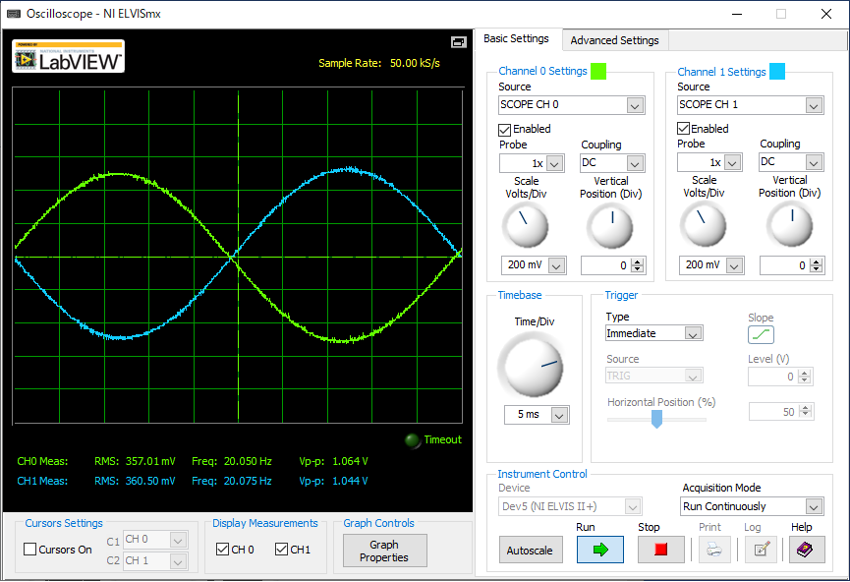
\includegraphics[width=0.8\linewidth]{src/figures/exp10/20k-20hz-sin.png}
		\subcaption{\SI{20}{Hz}}\label{fig:exp10-20hz}
	\end{subfigure}
	\begin{subfigure}{0.8\linewidth}
		\centering
		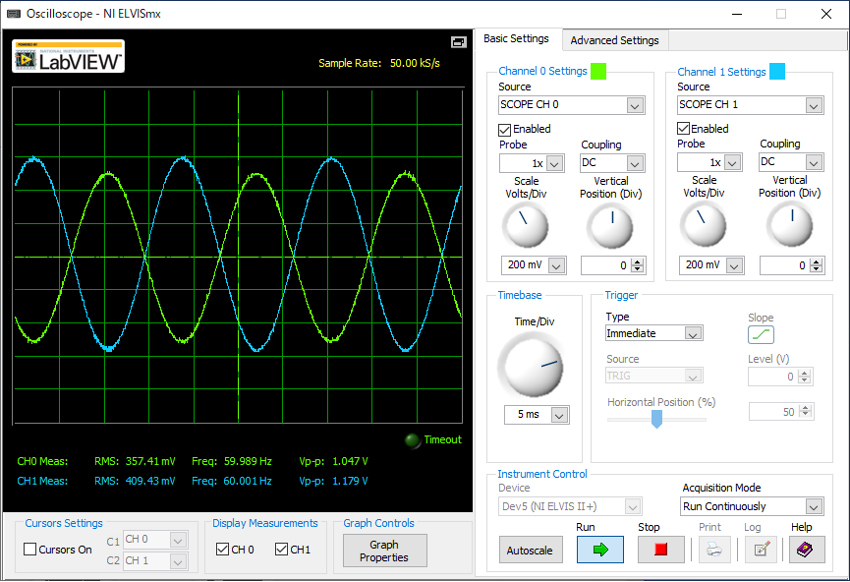
\includegraphics[width=0.8\linewidth]{src/figures/exp10/20k-60hz-sin.png}
		\subcaption{\SI{60}{Hz}}\label{fig:exp10-60hz}
	\end{subfigure}
\end{figure}
\begin{figure}
	\centering
	\begin{subfigure}{0.8\linewidth}
		\addtocontents{subfigure}{2}
		\centering
		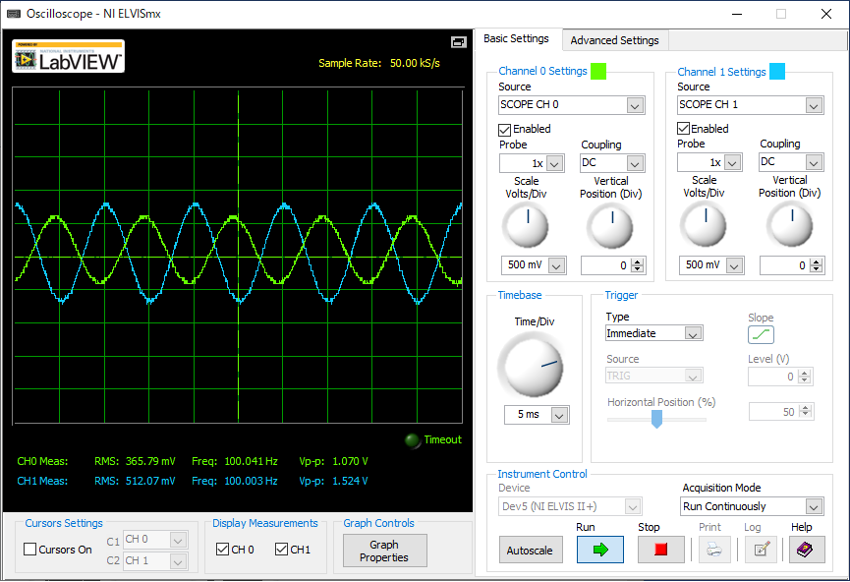
\includegraphics[width=0.8\linewidth]{src/figures/exp10/20k-100hz-sin.png}
		\subcaption{\SI{100}{Hz}}\label{fig:exp10-100hz}
	\end{subfigure}
	\begin{subfigure}{0.8\linewidth}
		\centering
		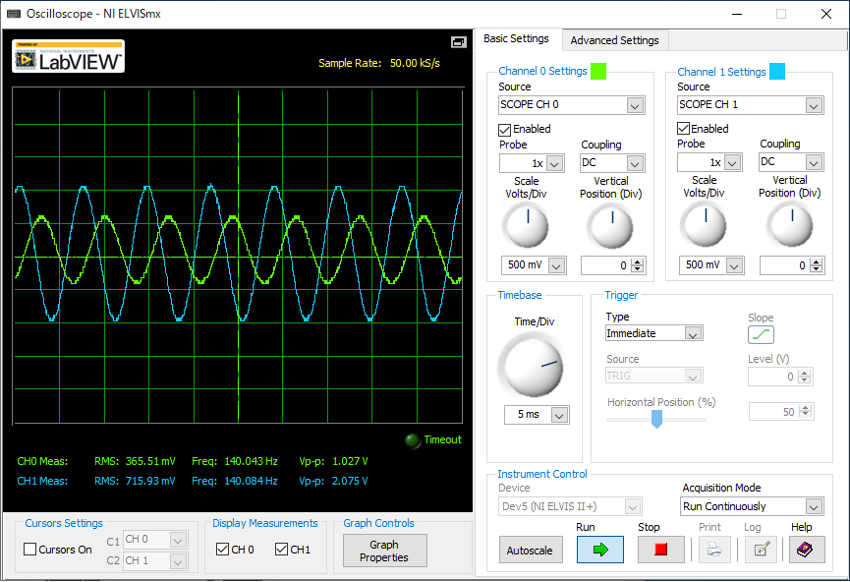
\includegraphics[width=0.8\linewidth]{src/figures/exp10/20k-140hz-sin.png}
		\subcaption{\SI{140}{Hz}}\label{fig:exp10-140hz}
	\end{subfigure}
\end{figure}
\begin{figure}
	\centering
	\begin{subfigure}{0.8\linewidth}
		\addtocounter{subfigure}{4}
		\centering
		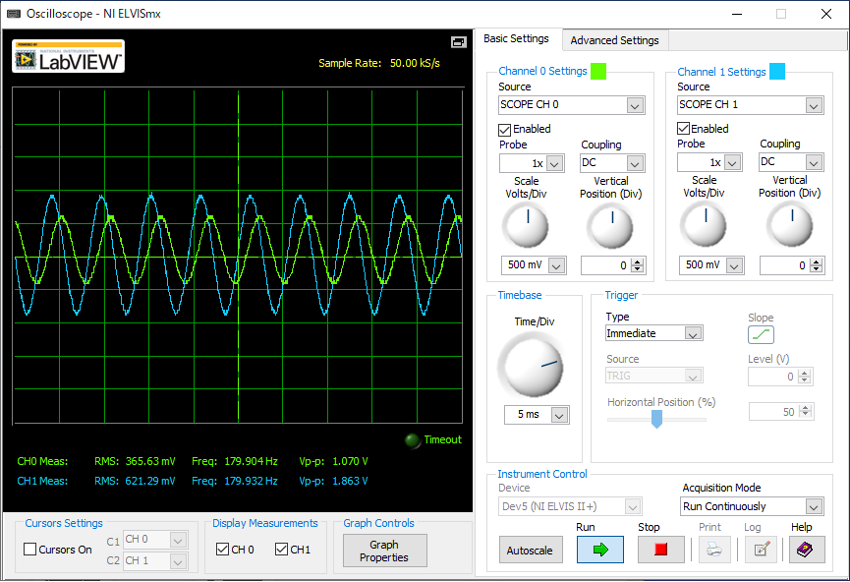
\includegraphics[width=0.8\linewidth]{src/figures/exp10/20k-180hz-sin.png}
		\subcaption{\SI{180}{Hz}}\label{fig:exp10-180hz}
	\end{subfigure}
	\caption{\SI{20}{Hz}から\SI{180}{Hz}まで\SI{40}{Hz}刻みで変化させたときの出力波形}\label{fig:exp10-band-sin}
\end{figure}
